\documentclass[12pt,a4paper]{report}
\usepackage[a4paper, margin=1in]{geometry}
\usepackage[utf8]{inputenc}
\usepackage{amsfonts}
\usepackage{amsmath}
\usepackage{amssymb}
\usepackage{setspace}
\usepackage{graphicx}
\usepackage{array}
\usepackage{fancyhdr}
\usepackage{ragged2e}
\linespread{1.5}
\usepackage{geometry}
\geometry{
a4paper,
total={210mm,297mm},
left=1.25in,
right=0.75in,
top=0.75in,
bottom=0.75in,
}
\usepackage{booktabs}
\usepackage{float}
\usepackage{placeins}
\usepackage{url}
\usepackage{hyperref}
\hypersetup{
    colorlinks=true,
    linkcolor=black,
    citecolor=black,
    urlcolor=black
}
\tolerance=1
\emergencystretch=\maxdimen
\hyphenpenalty=10000
\hbadness=10000

% --------------------------------------------------------------------------
% Project information
% --------------------------------------------------------------------------
\newcommand{\projecttitle}{An Explainable Federated Learning Framework for Privacy-Preserving Pneumonia Detection Using Chest X-ray Images}
\newcommand{\shorttitle}{Explainable Federated Learning for Pneumonia Detection}
\newcommand{\dept}{Computer Science and Engineering (Artificial Intelligence and Machine Learning)}
\newcommand{\college}{Sahyadri College of Engineering \& Management}
\newcommand{\guide}{Mrs.\ Rajeshwari R Shettigar}
\newcommand{\hod}{Dr.\ Pushpalatha K}
\newcommand{\principal}{Dr.\ S.\ S.\ Injaganeri}

\begin{document}
\pagestyle{empty}

% % ==========================================================================
% TITLE PAGE
% ==========================================================================

\thispagestyle{empty}

\begin{center}
{\large \textbf{VISVESVARAYA TECHNOLOGICAL UNIVERSITY}}
\par
{\large \textbf{``JNANA SANGAMA'', BELAGAVI - 590 018}}

\vspace{0.25cm}


\includegraphics[width=0.60in]{../fig/vtu}

\vspace{0.18cm}

\textbf{PROJECT PHASE-II REPORT}
\par

\vspace{0.04cm}

\textbf{on}
\par

\vspace{0.08cm}

{\Large \textbf{``\projecttitle''}}
\par

\vspace{0.12cm}

\textit{\textbf{Submitted by}}
\par

\vspace{0.005cm}

\end{center}

% Student details
\noindent
\begin{tabular}{p{6.0cm}p{4.0cm}}
\textbf{\large Arshith} & \textbf{\large 4SF23CI034} \\
\textbf{\large Manvith Kumar Ullal} & \textbf{\large 4SF23CI078} \\
\textbf{\large Preran Rai} & \textbf{\large 4SF23CI113} \\
\textbf{\large Thushar} & \textbf{\large 4SF24CI411}
\end{tabular}

\vspace{0.005cm}

\begin{center}

\textit{\textbf{In partial fulfillment of the requirements for the VII semester}}

\vspace{0.06cm}

\textbf{of}

\vspace{0.06cm}

{\large \textbf{BACHELOR OF ENGINEERING}}

\vspace{0.06cm}

\textbf{in}

\vspace{0.06cm}

{\large \textbf{COMPUTER SCIENCE AND ENGINEERING}}

\vspace{0.02cm}

\fontsize{13}{14}\selectfont
\textbf{(ARTIFICIAL INTELLIGENCE AND MACHINE LEARNING)}

\vspace{0.12cm}

\textit{\textbf{Under the Guidance of}}

\vspace{0.06cm}

\textbf{\guide}

\vspace{0.05cm}

\normalsize
\textbf{Assistant Professor, Department of CSE(AI\&ML)}

\vspace{0.12cm}

\textbf{at}

\vspace{0.08cm}


\includegraphics[width=0.9in]{../fig/Sahyadri}

\vspace{0.05cm}

{\LARGE \textbf{SAHYADRI}}

\vspace{0.03cm}

{\large \textbf{College of Engineering \& Management}}

\vspace{0.03cm}

{\large \textbf{An Autonomous Institution}}

\vspace{0.03cm}

{\large \textbf{MANGALURU}}

\vspace{0.03cm}

{\large \textbf{2026 -- 27}}

\end{center}

% ==========================================================================
% CERTIFICATE
% ==========================================================================
\newpage
\begin{center}
{\LARGE \textbf{SAHYADRI}}
\par
\vspace{3pt}
{\Large \textbf{College of Engineering \& Management}}
\par
\vspace{1pt}
{\large \textbf{An Autonomous Institution}}
\par
\vspace{1pt}
{\large \textbf{MANGALURU}}
\par
\vspace{0.015in}
\large \textbf{COMPUTER SCIENCE AND ENGINEERING}\\
\fontsize{13}{1}\textbf{(ARTIFICIAL INTELLIGENCE AND MACHINE LEARNING)}
\par

\begin{figure}[hbtp]
\centering
\includegraphics[width=1.0in,height=0.55in]{../fig/sahyadri}
\end{figure}

{\Large \textbf{CERTIFICATE}}
\end{center}

\par
\vspace{0.10in}
\setstretch{1.5}
\noindent
This is to certify that the \textbf{Project} entitled
\textbf{``\projecttitle''} has been carried out by
\textbf{Arshith (4SF23CI034), Manvith Kumar Ullal (4SF23CI078), Preran Rai (4SF23CI113)}
and \textbf{Thushar (4SF24CI411)}, the bonafide students of
\college\ in partial fulfillment of the requirements for the VII semester
\textbf{Project Work Phase-II (AM722P6A)} of \textbf{Bachelor of Engineering in
Computer Science and Engineering (AI\&ML)} of Visvesvaraya Technological
University, Belagavi during the year 2026--27. It is certified that all
corrections/suggestions indicated for Internal Assessment have been incorporated
in the report deposited in the departmental library. The project report has
been approved as it satisfies the academic requirements in respect of project
work Phase-II.

\begin{center}
\begin{tabular}{
>{\centering\arraybackslash}p{0.30\textwidth}
>{\centering\arraybackslash}p{0.30\textwidth}
>{\centering\arraybackslash}p{0.30\textwidth}
}
\underline{\hspace{3cm}} & \underline{\hspace{3cm}} & \underline{\hspace{3cm}} \\[0.15cm]
\textbf{Project Guide} & \textbf{HoD} & \textbf{Principal} \\[0.2cm]
\textbf{\guide} & \textbf{\hod} & \textbf{\principal}\\[0.15cm]
Dept.\ of CSE (AI\&ML) & Dept.\ of CSE (AI\&ML) & SCEM, Mangaluru
\end{tabular}
\end{center}

\vspace{0.25in}
\begin{center}
\textbf{External Viva-Voce}
\end{center}

\noindent
\textbf{Examiner's Name} \hfill \textbf{Signature with Date}

\vspace{0.5cm}
\noindent
1.\underline{\hspace{5cm}} \hfill \underline{\hspace{5cm}}

\vspace{0.5cm}
\noindent
2.\underline{\hspace{5cm}} \hfill \underline{\hspace{5cm}}

% ==========================================================================
% DECLARATION
% ==========================================================================
\newpage
\begin{center}
{\LARGE \textbf{SAHYADRI}}
\par
\vspace{6pt}
{\Large \textbf{College of Engineering \& Management}}
\par
\vspace{3pt}
{\large \textbf{An Autonomous Institution}}
\par
\vspace{3pt}
{\large \textbf{MANGALURU}}
\par
\vspace{0.25in}
{\large \textbf{Department of Computer Science and Engineering}\\
\fontsize{13}{1}\textbf{(Artificial Intelligence and Machine Learning)}}
\par

\begin{figure}[hbtp]
\centering
\includegraphics[width=1.25in,height=1in]{../fig/sahyadri}
\end{figure}

{\Large \textbf{DECLARATION}}
\end{center}

\par
\vspace{0.10in}
\setstretch{1.5}
\noindent
We hereby declare that the entire work embodied in this Project Report titled
\textbf{``\projecttitle''} has been carried out by us at \college,
Mangaluru under the supervision of \textbf{\guide} as part of the VII semester
\textbf{Project Work Phase-II (AM722P6A)} of \textbf{Bachelor of Engineering}
in \textbf{Computer Science and Engineering (AI\&ML)}. This report has not
been submitted to this or any other University.

\vspace{0.25in}
\begin{flushright}
\textbf{Arshith (4SF23CI034)}\\
\textbf{Manvith Kumar Ullal (4SF23CI078)}\\
\textbf{Preran Rai (4SF23CI113)}\\
\textbf{Thushar (4SF24CI411)}\\
SCEM, Mangaluru
\end{flushright}

% ==========================================================================
% ABSTRACT
% ==========================================================================
\newpage
\pagestyle{plain}
\pagenumbering{roman}

\chapter*{Abstract}
\addcontentsline{toc}{chapter}{\numberline{}Abstract}

Pneumonia remains a leading cause of hospitalization and mortality worldwide. Interpreting a chest X-ray for signs of pneumonia is a complex task, and variations in interpretation can often arise between different radiologists due to workload constraints and differing diagnostic thresholds. While deep learning models have shown tremendous potential in identifying subtle visual patterns indicative of pneumonia, conventional centralized training approaches demand that medical images from various hospitals be aggregated into a single repository. This centralized pooling approach fundamentally conflicts with strict patient privacy regulations and intricate institutional data-governance policies, rendering it highly impractical for real-world deployment.

To address these formidable challenges, this project introduces a robust explainable federated learning framework specifically tailored for privacy-preserving pneumonia detection. The proposed architecture eliminates the need to centralize sensitive patient data. Instead, a Squeeze-and-Excitation (SE) enhanced DenseNet121 model is trained collaboratively across three simulated hospital clients. During the federated training process, raw images remain securely on local servers; only the model parameters are securely transmitted and aggregated.

In this study, two distinct federated optimization strategies---FedAvg and FedProx---are rigorously evaluated under identical configurations to ascertain their respective strengths. Training and internal evaluations are performed utilizing the publicly available RSNA Pneumonia Detection Challenge dataset. To rigorously test the models' cross-domain generalization capabilities, an independent Labeled Chest X-ray Images dataset is employed for external evaluation without any prior fine-tuning.

Experimental results on the RSNA internal test set demonstrate that FedAvg achieves an accuracy of 82.49\% and an Area Under the ROC Curve (AUC) of 88.52\%. In contrast, FedProx attains an accuracy of 82.16\% and a marginally higher AUC of 88.63\%, while notably improving the recall from 73.28\% to 77.27\%. Crucially, the external evaluation highlights a significant divergence in robustness. While FedAvg suffers a severe drop in recall to 26.15\%, FedProx maintains a substantially higher recall of 54.62\% alongside an impressive F1-score of 69.84\% and an AUC of 90.35\%. This empirically validates that the proximal regularization inherent to FedProx effectively mitigates client drift, thereby enhancing generalizability across heterogeneous data distributions.

Furthermore, Grad-CAM (Gradient-weighted Class Activation Mapping) is integrated into the pipeline to foster trust and transparency. By generating visual heatmaps that highlight the specific clinically relevant lung regions influencing the model's predictions, the framework transitions from a "black-box" paradigm to a clinically interpretable diagnostic support tool. These findings underscore the immense potential of integrating attention-enhanced neural architectures with federated optimization and explainable AI, paving the way for scalable, privacy-preserving, and trustworthy collaborative medical imaging solutions.

% ==========================================================================
% ACKNOWLEDGEMENT
% ==========================================================================
\chapter*{Acknowledgement}
\addcontentsline{toc}{chapter}{\numberline{}Acknowledgement}

We take this opportunity to express our profound gratitude to everyone who supported us throughout the course of this project. The successful completion of this Project Report on \textbf{``\projecttitle''}, undertaken as a core component of the VII semester \textbf{Project Work Phase-II (AM722P6A)} for the \textbf{Bachelor of Engineering} in \textbf{Computer Science and Engineering (AI\&ML)} at Visvesvaraya Technological University, Belagavi, would not have been possible without their unwavering support.

\par
\vspace{0.15in}
\noindent
First and foremost, we express our sincere and heartfelt gratitude to our esteemed guide, \textbf{\guide}, Assistant Professor in the Department of Computer Science and Engineering (AI\&ML). Her deep technical insights, continuous encouragement, and patient mentorship have been instrumental in steering this research in the right direction. She provided invaluable feedback at every crucial juncture, ensuring that our methodology remained scientifically rigorous.

\par
\vspace{0.15in}
\noindent
We are immensely thankful to \textbf{\hod}, Professor and Head of the Department of Computer Science and Engineering (AI\&ML), for fostering an academic environment that encourages innovative thinking and for her steadfast support and administrative guidance throughout the academic year.

\par
\vspace{0.15in}
\noindent
We also wish to convey our deepest appreciation to our Principal, \textbf{\principal}, of \college, Mangaluru. We are grateful for the exceptional infrastructural facilities, computing resources, and the conducive academic atmosphere that the institution provided, all of which were vital to the execution of our experiments.

\par
\vspace{0.15in}
\noindent
Finally, we owe a deep debt of gratitude to our parents, family members, and friends. Their constant encouragement, moral support, and patience have been our source of strength during the challenging phases of this project.

\vspace{0.15in}
\begin{flushright}
\textbf{Arshith (4SF23CI034)}\\
\textbf{Manvith Kumar Ullal (4SF23CI078)}\\
\textbf{Preran Rai (4SF23CI113)}\\
\textbf{Thushar (4SF24CI411)}\\
VII Sem, B.E., CSE(AI\&ML)\\
SCEM, Mangaluru
\end{flushright}

% ==========================================================================
% TOC
% ==========================================================================
\setstretch{1.4}
\renewcommand{\contentsname}{Table of Contents}
\tableofcontents
\addcontentsline{toc}{chapter}{\numberline{}Table of Contents}
\listoffigures
\addcontentsline{toc}{chapter}{\numberline{}List of Figures}
\listoftables
\addcontentsline{toc}{chapter}{\numberline{}List of Tables}
\newpage

% ==========================================================================
% HEADER / FOOTER
% ==========================================================================
\pagestyle{fancy}
\fancyhf{}
\lhead{\fontsize{10}{12}\selectfont \shorttitle}
\rhead{\fontsize{10}{12}\selectfont Chapter \thechapter}
\lfoot{\fontsize{10}{12}\selectfont Department of CSE(AI\&ML), SCEM, Mangaluru}
\rfoot{\fontsize{10}{12}\selectfont Page \thepage}
\renewcommand{\headrulewidth}{0.5pt}
\renewcommand{\footrulewidth}{0.5pt}

\setstretch{1.5}
\justifying
\pagenumbering{arabic}
% ==========================================================================
% CHAPTER 1: INTRODUCTION
% ==========================================================================
\chapter{Introduction}

\section{Overview and Clinical Context}

Pneumonia continues to represent one of the most pervasive and formidable public health challenges across the globe, frequently resulting in prolonged hospital admissions and contributing significantly to mortality rates, particularly among vulnerable populations such as the elderly and immunocompromised individuals. In clinical practice, chest X-ray (CXR) imaging undeniably remains the first diagnostic tool that medical practitioners reach for. The widespread reliance on CXR stems from its unparalleled cost-effectiveness, rapid turnaround time, and near-universal availability, even in resource-constrained or remote medical facilities where advanced imaging modalities like CT scans or MRIs are scarce.

However, interpreting a chest radiograph is an inherently complex task that demands years of specialized medical training. The visual indicators of pulmonary infections, such as lung opacities, consolidations, or interstitial infiltrates, can often be exceedingly subtle and easily obscured by the complex underlying anatomical structures of the thorax, such as the rib cage, clavicles, and the heart shadow. Consequently, even experienced radiologists can differ in their interpretations. This inter-observer variability can be further exacerbated by factors such as high patient volume, clinician fatigue, and suboptimal image quality. It is precisely this gap between the necessity for rapid, accurate diagnosis and the human limitations of manual interpretation that has propelled the rapid evolution of computer-aided diagnosis (CAD) systems. The overarching goal of these systems is not to render the human radiologist obsolete, but rather to serve as a highly reliable, tireless second reader that flags potential anomalies and prioritizes urgent cases.

Convolutional Neural Networks (CNNs) have emerged as an exceptionally potent architecture for this specific task. Unlike traditional machine learning approaches that necessitate tedious and often fragile manual feature extraction, CNNs have the innate ability to autonomously learn hierarchical visual features directly from raw pixel data. Among the myriad of CNN architectures, DenseNet121 has distinguished itself as a particularly well-suited choice for radiographic image analysis. Its defining characteristic---the dense connectivity pattern where each layer receives direct inputs from all preceding layers within a dense block---encourages extensive feature reuse. This design elegantly circumvents the vanishing gradient problem and ensures that both low-level morphological details and high-level abstract features are preserved throughout the network. Crucially, this efficiency translates to a comparatively lower parameter count, allowing the network to achieve state-of-the-art representational power without the exorbitant computational overhead or the severe risk of overfitting associated with deeper, more traditional networks. The seminal work on CheXNet definitively proved that a DenseNet-based architecture could identify pneumonia and other thoracic pathologies from chest X-rays at a proficiency level comparable to practicing radiologists, thereby establishing a robust benchmark for all subsequent research in this domain \cite{rajpurkar2017chexnet,huang2017densely}.

Despite these monumental algorithmic strides, the practical deployment of deep learning pipelines in the healthcare sector is frequently paralyzed by a fundamental operational assumption: the necessity of centralized data pooling. Most state-of-the-art models are trained under the premise that massive volumes of patient data from diverse hospitals can be aggregated into a single, monolithic repository. In reality, this centralized paradigm aggressively conflicts with a labyrinth of patient privacy regulations (such as HIPAA in the United States or the GDPR in Europe), stringent institutional data-governance policies, and the justifiable reluctance of healthcare providers to relinquish control over their proprietary medical records. 

Federated Learning (FL) presents an elegant and robust paradigm shift that neatly sidesteps this data siloing problem. Instead of moving the sensitive patient data to a centralized server where the model resides, FL distributes the model to the dispersed client institutions where the data securely resides \cite{mcmahan2017communication,rieke2020,sheller2020federated}. In a standard FL setup, the central aggregation server initiates the process by dispatching a global model to participating clients. Each client then independently trains the model on its private, localized dataset for a predetermined number of epochs. Following this local training phase, the clients transmit only their updated model parameters (or weight differentials) back to the central server. The server then aggregates these disparate updates to synthesize a refined global model. This iterative process continues across multiple communication rounds until the model converges. The most ubiquitous aggregation algorithm, Federated Averaging (FedAvg), computes a straightforward weighted average of the client parameters. While remarkably communication-efficient, FedAvg is notorious for suffering performance degradation when the data distributed across clients is heavily heterogeneous, or non-IID (Independent and Identically Distributed)---a scenario that perfectly characterizes the fragmented reality of medical data. To counteract this, more sophisticated optimization strategies like FedProx introduce a proximal regularization term into the local client objective function, mathematically penalizing the local model if it drifts excessively far from the global consensus \cite{li2020federated}.

Yet, overcoming the data privacy hurdle solves only half of the clinical adoption puzzle. A decentralized, privacy-preserving model that functions as an impenetrable "black box"---yielding only a probability score without any contextual justification---is of little practical utility to a clinician responsible for patient care. Explainable Artificial Intelligence (XAI) bridges this critical trust deficit. Techniques such as Gradient-weighted Class Activation Mapping (Grad-CAM) are indispensable in this regard. Grad-CAM leverages the gradients of the target concept flowing into the final convolutional layer to generate a coarse localization map, effectively highlighting the precise anatomical regions in the image that most heavily influenced the network's final prediction \cite{selvaraju2017gradcam}. By harmonizing federated training architectures with visual interpretability, this project proposes a comprehensive, end-to-end framework that is simultaneously privacy-aware, clinically transparent, and diagnostically potent.

The core computational engine driving this research is an ImageNet-pretrained DenseNet121 architecture, strategically augmented with Squeeze-and-Excitation (SE) attention mechanisms. These SE blocks dynamically recalibrate the channel-wise feature responses, effectively teaching the network to selectively amplify informative feature maps while suppressing irrelevant background noise \cite{hu2018squeeze}. This SE-DenseNet121 model is rigorously trained across three simulated hospital nodes using both the standard FedAvg and the advanced FedProx optimization strategies. The framework undergoes internal evaluation utilizing the benchmark RSNA Pneumonia Detection Challenge dataset, followed by a stringent external evaluation phase on the fully independent Labeled Chest X-ray Images dataset to objectively measure true cross-domain generalizability.

\section{Purpose and Motivation}

The primary motivation behind this research endeavor is to architect and critically evaluate a federated deep learning framework explicitly designed for automated pneumonia detection, one that unconditionally respects patient privacy by ensuring that raw chest X-ray images never traverse the network. A central, guiding inquiry of this project is to ascertain whether this decentralized, collaborative training methodology can genuinely rival the diagnostic accuracy achieved by conventional centralized training methods. Furthermore, this study seeks to empirically determine if the proximal regularization introduced by FedProx provides a tangible, measurable advantage over the standard FedAvg algorithm, particularly when confronted with the statistical heterogeneity that is inevitable in real-world clinical datasets.

A secondary, equally critical purpose is to dismantle the opaque nature of deep neural networks, making their internal decision-making processes transparent and trustworthy for medical professionals. By systematically generating and analyzing Grad-CAM visualizations for a variety of cases---encompassing true positives, true negatives, and crucially, misclassifications---the project aims to provide direct, visual evidence of the model's focus. This ensures that the model's diagnostic conclusions are driven by genuine pathological indicators rather than artifactual noise or confounding variables present in the scans. Ultimately, this project approaches diagnostic accuracy, decentralized data privacy, and clinical interpretability not as isolated technical challenges, but as deeply intertwined facets of a singular, holistic healthcare AI solution.

\section{Scope of the Project}

The precise scope of this project is constrained to the binary classification of pneumonia from chest X-ray images utilizing a sophisticated SE-enhanced DenseNet121 backbone. The extensive RSNA Pneumonia Detection Challenge dataset serves as the foundational data source for model development, hyperparameter tuning, and internal validation. Crucially, a completely separate and independent Labeled Chest X-ray Images dataset is rigorously reserved exclusively for external evaluation, simulating a real-world deployment scenario to test the model's resilience to previously unseen data distributions. The federated architecture is actualized through the instantiation of three simulated hospital clients.

In granular detail, the scope encompasses the following sequential phases:
\begin{itemize}
    \item \textbf{Data Curation and Preprocessing:} Implementing robust pipelines for decoding, standardizing, and applying clinically appropriate stochastic augmentations to chest X-ray images to enhance model robustenss.
    \item \textbf{Architectural Engineering:} Leveraging transfer learning via an ImageNet-pretrained DenseNet121 network, and seamlessly integrating Squeeze-and-Excitation (SE) attention mechanisms to refine feature extraction capabilities.
    \item \textbf{Federated Optimization:} Constructing a decentralized training environment and meticulously implementing both the FedAvg and FedProx aggregation algorithms under strictly controlled and identical hyperparameter configurations to ensure a fair comparative analysis.
    \item \textbf{Comprehensive Evaluation:} Conducting multifaceted evaluations, calculating metrics including accuracy, precision, recall, F1-score, and AUC-ROC, alongside generating detailed confusion matrices and Receiver Operating Characteristic (ROC) curves.
    \item \textbf{Cross-Domain Generalization:} Executing zero-shot external evaluations on an independent dataset to definitively measure the models' robustness against domain shifts without any post-training fine-tuning.
    \item \textbf{Explainability Integration:} Generating, overlaying, and analyzing Grad-CAM heatmaps to visually interpret the spatial representations driving the model's diagnostic predictions.
\end{itemize}

It is equally important to meticulously define what falls outside the scope of this research. While the framework mimics a decentralized network, the three client nodes are simulated data partitions derived from a central dataset, rather than physically distinct hospital servers distributed across a wide area network. Consequently, the intricacies of real-world network latency and asynchronous communication protocols are abstracted. Furthermore, while the federated approach inherently safeguards raw data, implementing cryptographic privacy guarantees such as formal Differential Privacy (DP), Secure Multiparty Computation (SMPC), or Homomorphic Encryption falls outside the current scope, although these are recognized as essential future enhancements.

\section{Problem Statement}

The contemporary landscape of medical AI is dominated by centralized models that require the vast aggregation of patient data from disparate institutions into a singular computational silo. This aggregation prerequisite triggers a cascade of severe privacy, ethical, and legal complications, often creating insurmountable barriers to inter-institutional collaboration. Furthermore, even when data is successfully aggregated, the deep learning models deployed often function as opaque mathematical black boxes. When a model outputs a probability indicating the presence of pneumonia, a clinician is left without any mechanistic or visual explanation of how that conclusion was formulated, severely undermining clinical trust and hindering adoption.

The imperative, therefore, is the development of an advanced computational framework capable of collaboratively training a highly accurate pneumonia detection model without ever mandating the transfer of raw, sensitive chest X-ray data from the host institutions. This framework must not only guarantee data localization but also inherently provide interpretable, visual justifications for its diagnostic outputs. Crucially, the system must demonstrate robust resilience against the statistical heterogeneity endemic to different hospital datasets, and prove its capability to generalize reliably to entirely unseen patient populations. The central problem is discovering whether advanced federated optimization techniques, specifically FedProx, can demonstrably bridge the generalization gap often observed in standard federated averaging, while simultaneously maintaining clinical transparency through attention mechanisms.

\section{Objectives}

To systematically address the problem statement, this project is guided by the following explicit objectives:
\begin{enumerate}
    \item \textbf{Model Formulation:} To meticulously engineer and optimize an SE-enhanced DenseNet121 deep neural network explicitly tailored for the binary classification of pneumonia from complex chest X-ray imagery.
    \item \textbf{Federated Infrastructure:} To architect and deploy a simulated federated learning ecosystem comprising three distinct, non-overlapping hospital clients, ensuring that raw patient data remains strictly localized during all phases of training.
    \item \textbf{Algorithmic Comparison:} To implement, execute, and rigorously compare the performance of the FedAvg and FedProx optimization algorithms under rigorously matched experimental conditions to isolate their respective efficacies.
    \item \textbf{Internal Validation:} To comprehensively quantify the internal diagnostic performance of the global models utilizing a robust suite of metrics, including accuracy, precision, recall, F1-score, and Area Under the ROC Curve (AUC-ROC).
    \item \textbf{Generalization Assessment:} To objectively evaluate the cross-domain generalization capabilities of the synthesized global models by executing external evaluations on an independent, unseen Labeled Chest X-ray Images dataset, strictly without any supplementary fine-tuning.
    \item \textbf{Visual Interpretability:} To systematically implement Gradient-weighted Class Activation Mapping (Grad-CAM) to generate clinically meaningful visual explanations, elucidating the specific anatomical features dictating the model's predictions and thereby fostering clinical trust.
\end{enumerate}

\section{Organization of the Report}

The remainder of this comprehensive project report is structured systematically into seven subsequent chapters, each detailing a critical phase of the research. Chapter 2 provides an exhaustive review of the relevant academic literature, tracing the evolution of deep learning in radiographic analysis, the genesis of federated learning, and the imperative for explainable AI. Chapter 3 delves deep into the mathematical formulation of the problem, detailing the optimization objectives and the theoretical underpinnings of the chosen algorithms. Chapter 4 explicitly outlines the hardware and software prerequisites, along with the functional and non-functional requirements that governed the system's design. Chapter 5 offers a granular breakdown of the system architecture, detailing the implementation nuances of the preprocessing pipelines, the network design, and the federated workflows. Chapter 6 presents a rigorous, multifaceted analysis of the experimental results, interpreting the data through the lenses of statistical performance and clinical relevance. Chapter 7 synthesizes the overarching conclusions drawn from the research, candidly acknowledging the project's limitations. Finally, Chapter 8 charts a strategic course for future research, identifying key areas for enhancement and real-world deployment.

% ==========================================================================
% CHAPTER 2: LITERATURE REVIEW
% ==========================================================================
\chapter{Literature Review}

\noindent
The methodological foundations of this research are built upon the convergence of three distinct yet highly complementary technological domains: the application of sophisticated Deep Learning architectures for high-resolution chest X-ray analysis, the deployment of Federated Learning (FL) frameworks to enable decentralized, privacy-preserving model training, and the integration of Explainable Artificial Intelligence (XAI) to ensure the clinical interpretability of the resultant predictive models. This chapter provides an exhaustive exploration of the historical progression, current state-of-the-art, and identified limitations within these intersecting fields.

\section{Evolution of Deep Learning in Chest Radiography}

The landscape of medical image analysis has undergone a paradigm shift over the past decade, transitioning from reliance on human-engineered, handcrafted feature extraction techniques to the adoption of fully automated, end-to-end representation learning through Deep Convolutional Neural Networks (CNNs). Early attempts at computer-aided diagnosis often struggled with the vast inter-patient anatomical variability and the subtle, diffuse nature of pulmonary pathologies visible in chest X-rays.

The introduction of the DenseNet architecture by Huang et al. marked a watershed moment in computer vision, proving exceptionally relevant for medical imaging \cite{huang2017densely}. The defining innovation of DenseNet121 lies in its dense connectivity pattern; within each dense block, every convolutional layer is directly connected to all subsequent layers. This architectural choice fundamentally alters the flow of information and gradients through the network. By concatenating feature maps rather than summing them (as seen in ResNet architectures), DenseNet enforces aggressive feature reuse. This ensures that critical low-level textural features---which are often vital for identifying subtle pulmonary infiltrates---are not lost in the deeper layers of the network. Furthermore, this implicit deep supervision dramatically mitigates the vanishing gradient problem and results in a highly parameter-efficient model, which is crucial when training on medical datasets that are inherently constrained in size compared to massive natural image datasets.

Building upon this formidable foundation, Rajpurkar et al. developed CheXNet, a monumental leap in the domain of automated radiographic analysis \cite{rajpurkar2017chexnet}. By training a 121-layer DenseNet on the massive ChestX-ray14 dataset, they demonstrated that a deep learning algorithm could not only detect pneumonia but could do so with an F1 metric that statistically exceeded the performance of practicing radiologists. This research definitively established DenseNet121 as the gold standard backbone for thoracic disease classification. Subsequently, the RSNA Pneumonia Detection Challenge provided the research community with a meticulously curated, expert-annotated benchmark dataset, catalyzing further innovations and standardizing the evaluation of pneumonia detection algorithms \cite{shih2019rsna}.

However, a critical, unifying limitation pervades this impressive lineage of research: the fundamental assumption of data centralization. The extraordinary performance of models like CheXNet was predicated on the availability of massive, monolithic repositories of patient data. As AI research intersects with the realities of clinical deployment, this assumption shatters against the bedrock of medical privacy laws, ethical data stewardship, and institutional proprietary boundaries, necessitating a fundamental rethinking of how medical models are trained.

\section{Attention Mechanisms and Feature Recalibration}

While CNNs are adept at extracting hierarchical spatial features, standard convolutional operations treat all feature channels within a given layer with equal importance. In the context of chest radiography, this is suboptimal; the visual evidence defining a pathology like pneumonia may be highly localized to a specific region (e.g., a consolidation in the lower left lobe) and represented strongly in only a subset of feature channels, while the rest of the image contains irrelevant background anatomy.

To address this inefficiency, Hu et al. introduced Squeeze-and-Excitation (SE) networks, introducing the concept of channel-wise attention \cite{hu2018squeeze}. An SE block acts as a lightweight, computational module that dynamically recalibrates channel-wise feature responses. The process operates in two distinct phases: 'Squeeze' and 'Excitation'. The 'Squeeze' operation employs global average pooling to aggregate spatial dimensions, distilling the global spatial information of each channel into a singular, representative numeric descriptor. The 'Excitation' phase then passes these descriptors through a small bottleneck fully connected network, which learns the nonlinear interactions and dependencies between channels. The output is a set of modulation weights (ranging between 0 and 1 via a sigmoid activation) that are multiplied back into the original feature maps.

By integrating SE blocks into the DenseNet architecture, the network gains the adaptive capacity to selectively emphasize informative, pathology-relevant channels while actively suppressing noise or uninformative channels. This attention mechanism is particularly potent in medical imaging, where improving the signal-to-noise ratio at the feature level directly translates to higher diagnostic precision and a reduction in false-positive predictions.

\section{The Advent of Federated Learning in Healthcare}

Federated Learning (FL) was first conceptualized by McMahan et al. at Google as a novel distributed machine learning paradigm designed to train models on mobile devices without uploading user data to central servers \cite{mcmahan2017communication}. The fundamental premise of FL is bringing the code to the data, rather than the data to the code.

The healthcare sector, plagued by data fragmentation and stringent privacy regulations like HIPAA and GDPR, quickly recognized FL as a transformative solution. Rieke et al. provided a comprehensive overview of how FL could revolutionize digital health by enabling multi-institutional collaborations that were previously legally or logistically impossible \cite{rieke2020}. By allowing hospitals to train models collaboratively while keeping their sensitive patient records strictly within their own secure firewalls, FL circumvents the need for data sharing agreements and minimizes the risk of catastrophic data breaches.

Sheller et al. provided one of the first major empirical validations of this concept in the medical domain, demonstrating that a model trained via federated learning across multiple institutions could achieve performance on par with a model trained on centrally pooled data, all without compromising patient privacy \cite{sheller2020federated}. Furthermore, Kaissis et al. contextualized federated learning within a broader taxonomy of privacy-enhancing technologies, emphasizing that FL is a foundational pillar upon which highly secure medical AI ecosystems must be built \cite{kaissis2020secure}.

It is critical, however, to acknowledge the nuances of FL privacy. While FL fundamentally protects raw patient images, the model parameters or gradients transmitted over the network are not completely devoid of information. Advanced adversarial attacks, such as model inversion or membership inference attacks, have demonstrated that it is theoretically possible to reverse-engineer certain characteristics of the training data from the weight updates. Therefore, FL is often viewed as the first, albeit most critical, layer of defense, frequently requiring augmentation with additional cryptographic techniques for absolute security.

\section{Federated Optimization: The Challenge of Heterogeneity}

The default algorithm driving most federated networks is Federated Averaging (FedAvg), introduced alongside the FL concept by McMahan et al. \cite{mcmahan2017communication}. FedAvg is elegant in its simplicity: each client performs multiple steps of Stochastic Gradient Descent (SGD) locally, and the server computes a weighted average of the resulting models. When the data distributed across clients is Independent and Identically Distributed (IID), FedAvg converges rapidly and efficiently.

However, medical data is notoriously non-IID. Different hospitals employ different imaging equipment, adhere to varying acquisition protocols, serve demographically distinct patient populations, and may exhibit drastically different disease prevalence rates. This statistical heterogeneity causes a phenomenon known as "client drift," where each local model overfits to its specific data distribution and drifts away from the optimal global consensus. When these divergent models are averaged by the server, the resulting global model often suffers from degraded performance and slow convergence.

To directly combat this challenge, Li et al. proposed FedProx, a generalized and more robust optimization framework \cite{li2020federated}. FedProx tackles statistical heterogeneity by modifying the local objective function at each client. It introduces a proximal regularization term that mathematically restricts the local updates from diverging too significantly from the current global model provided by the server. This proximal term acts as an anchor, ensuring that while the client learns from its local data, it remains tethered to the collective knowledge of the federation. Given the inherent variability in multi-institutional chest X-ray datasets, investigating the comparative efficacy of FedProx versus FedAvg is a central focus of this research, addressing a critical gap in the practical deployment of medical FL systems.

\section{Demystifying Decisions with Explainable AI (XAI)}

The exceptional predictive accuracy of deep neural networks is frequently overshadowed by their "black-box" nature. In high-stakes domains like healthcare, providing a clinician with a binary diagnosis devoid of supporting evidence is unacceptable and often leads to the rejection of the AI tool. Clinicians require interpretability to verify that the model's logic aligns with established medical knowledge and is not relying on spurious correlations (e.g., learning to identify a specific hospital's watermark rather than the pathology).

Explainable AI (XAI) encompasses a suite of techniques designed to shed light on model behavior. For convolutional networks, Gradient-weighted Class Activation Mapping (Grad-CAM), developed by Selvaraju et al., has become the standard technique for post-hoc visual explanation \cite{selvaraju2017gradcam}. Grad-CAM does not require any architectural modifications or re-training. Instead, it utilizes the gradients of the target class score flowing into the final convolutional layer to calculate the importance weights of each feature map. By computing a weighted combination of these feature maps and passing them through a ReLU activation (to isolate features that positively influence the target class), Grad-CAM generates a coarse localization heatmap.

When overlaid on the original chest radiograph, this heatmap provides immediate visual feedback. If the model predicts pneumonia, a clinician can instantly verify if the heatmap highlights clinically relevant pulmonary opacities or consolidations. Conversely, if the model incorrectly focuses on the clavicle or medical tubing, the clinician can safely discount the prediction. In this project, Grad-CAM is deployed not just as an analytical tool, but as a crucial mechanism for building clinical trust in the federated model's outputs.

\section{The Imperative of Cross-Domain Generalization}

A pervasive flaw in much of the applied machine learning literature is the over-reliance on intra-dataset evaluation. A model that achieves stellar metrics on a held-out test set drawn from the same distribution as its training data may still fail catastrophically when deployed in a new hospital. Differences in scanner calibration, patient positioning, and image reconstruction algorithms can introduce subtle domain shifts that the model has never encountered.

In medical AI, the true measure of a model's utility is its cross-domain generalization capability. This refers to the model's robustness when evaluated on an entirely independent, geographically or temporally distinct dataset. In this project, the Labeled Chest X-ray Images dataset serves this precise purpose. By evaluating the federated models on this external dataset without any fine-tuning, the research rigorously tests whether the learned representations are genuinely invariant to domain shifts. This external validation is critical for answering whether federated optimization strategies like FedProx not only handle local heterogeneity but also confer broader generalizability to unseen data distributions.

\section{Summary and Identification of the Research Gap}

The literature demonstrates mature, well-established silos of research: CNNs for image analysis, FL for distributed training, and Grad-CAM for interpretability. However, a significant research gap exists at the intersection of these domains. Very few studies have attempted to integrate attention-enhanced CNN architectures, robust federated optimization algorithms (specifically comparing FedAvg and FedProx), and explainable AI within a unified, end-to-end framework dedicated to pneumonia detection. 

Furthermore, the majority of federated learning studies in medical imaging conclude their analysis upon evaluating internal test sets. This project deliberately addresses these gaps by architecting a comprehensive SE-DenseNet121 federated framework, rigorously evaluating the impact of proximal regularization under simulated heterogeneity, and, most importantly, extending the evaluation protocol to include stringent cross-dataset validation to truly measure real-world clinical applicability.

\begin{table}[H]
\centering
\caption{Comprehensive Summary of Foundational Literature}
\label{tab:literature_summary}
\begin{tabular}{p{3.0cm}p{3.5cm}p{6.5cm}}
\toprule
\textbf{Author(s) \& Year} & \textbf{Technological Area} & \textbf{Core Contribution and Relevance} \\
\midrule
Huang et al. (2017) & CNN Architectures & Introduced DenseNet, proving that dense connectivity maximizes feature reuse and mitigates vanishing gradients.\\
Rajpurkar et al. (2017) & Radiographic AI & Developed CheXNet, establishing the viability of DenseNet for radiologist-level pneumonia detection.\\
McMahan et al. (2017) & Federated Learning & Pioneered the FL paradigm and the FedAvg algorithm for decentralized, privacy-preserving model training.\\
Li et al. (2020) & Federated Optimization & Introduced FedProx, utilizing proximal regularization to handle statistical heterogeneity and limit client drift.\\
Hu et al. (2018) & Attention Mechanisms & Developed Squeeze-and-Excitation (SE) networks for adaptive, channel-wise feature recalibration.\\
Selvaraju et al. (2017) & Explainable AI (XAI) & Created Grad-CAM, enabling gradient-based visual localization of CNN predictions without architectural changes.\\
Rieke et al. (2020) & FL in Healthcare & Outlined the strategic vision for FL as the foundational architecture for collaborative digital health networks.\\
Sheller et al. (2020) & Applied Medical FL & Provided empirical evidence that FL can train multi-institutional medical models without compromising patient data.\\
\bottomrule
\end{tabular}
\end{table}
% ==========================================================================
% CHAPTER 3: PROBLEM FORMULATION
% ==========================================================================
\chapter{Problem Formulation}

\section{System Architecture and Data Distribution}

Consider a distributed healthcare consortium comprising $K$ distinct and independent participating hospitals, mathematically represented as clients $C_1, C_2, \ldots, C_K$. Each client $C_k$ possesses a localized, private repository of medical data, denoted as $D_k = \{(x_i, y_i)\}_{i=1}^{n_k}$. In this formulation, $x_i \in \mathbb{R}^{C \times H \times W}$ represents a chest X-ray image (where $C$ is the number of channels, and $H, W$ are the spatial dimensions), and $y_i \in \{0, 1\}$ represents the corresponding binary ground-truth label, where 0 indicates a normal radiograph and 1 indicates the presence of pneumonia. The total number of training samples across the entire federation is $n = \sum_{k=1}^{K} n_k$.

The fundamental constraint of this federated ecosystem is strict data localization: no raw image data $x_i$ or label $y_i$ is permitted to leave the premises of client $C_k$. The central objective is to collaboratively learn a global parameterized model, defined by its weight vector $w \in \mathbb{R}^d$, that achieves high predictive accuracy across the global data distribution without violating this privacy constraint.

\section{The Federated Optimization Objective}

In a conventional, centralized machine learning paradigm, the objective is to find a weight vector $w$ that minimizes the empirical risk over the entire dataset. In the federated paradigm, this global objective is decomposed into a weighted sum of local objectives. The global loss function $F(w)$ that the federation seeks to minimize is mathematically formulated as:

\begin{equation}
\min_w F(w) = \sum_{k=1}^{K} \frac{n_k}{n} F_k(w),
\end{equation}

where $F_k(w)$ represents the local empirical risk on client $k$'s private dataset $D_k$. The weighting factor $\frac{n_k}{n}$ ensures that the global model is proportionally influenced by the volume of data held by each client, preventing clients with negligible data from exerting undue influence on the global parameters.

\subsection{Local Binary Classification Objective}

Given the binary nature of the pneumonia detection task, the local objective $F_k(w)$ is optimized using a Binary Cross-Entropy (BCE) loss formulation. However, medical datasets are inherently imbalanced; normal cases frequently outnumber pathological cases. To prevent the model from becoming biased toward the majority class, a class-weighted BCE is employed. For a given sample $(x, y)$ and the model's predicted probability $\hat{y} = f(x; w)$, the loss is defined as:

\begin{equation}
\mathcal{L}_{BCE}(y, \hat{y}) = - \left[ w_{pos} \cdot y \log(\hat{y}) + w_{neg} \cdot (1-y) \log(1-\hat{y}) \right],
\end{equation}

where $w_{pos}$ and $w_{neg}$ are the statistical weights assigned to the positive (pneumonia) and negative (normal) classes, respectively, calculated inversely proportional to their class frequencies in the dataset.

\section{Federated Aggregation Algorithms}

To optimize the global objective $F(w)$ in a decentralized manner, iterative communication rounds between the central server and the clients are required. This project investigates and compares two distinct optimization strategies.

\subsection{Federated Averaging (FedAvg)}

FedAvg is the baseline aggregation protocol. At communication round $t$, the central server broadcasts the current global model $w^t$ to the clients. Each client $k$ initializes its local model with $w^t$ and performs $E$ epochs of stochastic gradient descent (SGD) to minimize its local objective $F_k(w)$, yielding updated local parameters $w_k^{t+1}$. The server then aggregates these local updates to form the new global model:

\begin{equation}
w^{t+1} = \sum_{k=1}^{K} \frac{n_k}{n} w_k^{t+1}.
\end{equation}

While computationally efficient, FedAvg assumes that the local objectives $F_k(w)$ are relatively homogeneous approximations of the global objective $F(w)$. When data is non-IID, this assumption fails, leading to client drift.

\subsection{Federated Proximal Optimization (FedProx)}

To mitigate the divergence caused by statistical heterogeneity, FedProx alters the local optimization landscape. It introduces a proximal regularization term to the local objective function at each client. At round $t$, client $k$ seeks to minimize a modified local function $h_k(w)$:

\begin{equation}
\min_w h_k(w) = F_k(w) + \frac{\mu}{2} \left\| w - w^t \right\|^2.
\end{equation}

The proximal term $\frac{\mu}{2} \| w - w^t \|^2$ serves as a penalty that restricts the updated local parameters $w$ from moving too far away from the current global consensus model $w^t$. The hyperparameter $\mu > 0$ controls the intensity of this restriction. In our experimental setup, $\mu$ is empirically set to 0.01. Once local training is complete, the server aggregates the parameters identically to FedAvg.

\section{Mathematical Formulation of the Attention Mechanism}

The chosen model architecture incorporates Squeeze-and-Excitation (SE) blocks to facilitate dynamic feature recalibration. Let $\mathbf{U} \in \mathbb{R}^{C \times H \times W}$ represent an intermediate feature map generated by a convolutional block, where $C$ is the number of feature channels.

The \textbf{Squeeze} operation aggregates spatial information across the $H \times W$ dimensions to produce a channel-wise descriptor $\mathbf{z} \in \mathbb{R}^C$. This is achieved via Global Average Pooling (GAP):

\begin{equation}
z_c = \frac{1}{H \times W} \sum_{i=1}^{H} \sum_{j=1}^{W} u_c(i,j), \quad \text{for } c = 1, \dots, C.
\end{equation}

The \textbf{Excitation} operation captures channel-wise dependencies using a bottleneck architecture composed of two fully connected (FC) layers. The descriptor $\mathbf{z}$ is transformed to generate a modulation weight vector $\mathbf{s} \in \mathbb{R}^C$:

\begin{equation}
\mathbf{s} = \sigma\left( \mathbf{W}_2 \delta( \mathbf{W}_1 \mathbf{z} ) \right),
\end{equation}

where $\mathbf{W}_1 \in \mathbb{R}^{\frac{C}{r} \times C}$ acts as a dimensionality reduction layer (with reduction ratio $r$), $\delta$ represents the ReLU activation function, $\mathbf{W}_2 \in \mathbb{R}^{C \times \frac{C}{r}}$ acts as a dimensionality increasing layer, and $\sigma$ represents the sigmoid activation function, constraining the weights to the $[0, 1]$ interval.

Finally, the recalibrated feature map $\widetilde{\mathbf{U}}$ is obtained by scaling the original feature map $\mathbf{U}$ with the learned activations $\mathbf{s}$:

\begin{equation}
\tilde{u}_c = s_c \cdot u_c.
\end{equation}

\section{Formulation of Visual Explainability (Grad-CAM)}

To render the model's predictions interpretable, Gradient-weighted Class Activation Mapping (Grad-CAM) is mathematically formulated to identify discriminative regions. Let $y^c$ represent the raw predicted score (before the sigmoid activation) for the target class $c$ (pneumonia). Let $A^k \in \mathbb{R}^{H' \times W'}$ represent the $k$-th feature map activation of the final convolutional layer.

First, the gradients of the score $y^c$ with respect to the feature map activations $A^k$ are computed. These gradients are then globally averaged over the spatial dimensions to obtain the neuron importance weights $\alpha_k^c$:

\begin{equation}
\alpha_k^c = \frac{1}{Z} \sum_{i} \sum_{j} \frac{\partial y^c}{\partial A_{ij}^k},
\end{equation}

where $Z = H' \times W'$ is the total number of pixels in the feature map. These weights $\alpha_k^c$ represent a partial linearization of the deep network downstream from $A$, capturing the 'importance' of feature map $k$ for a target class $c$.

The final Grad-CAM heatmap, $L_{\mathrm{Grad-CAM}}^c$, is generated by computing a weighted linear combination of the forward activation maps, followed by a ReLU activation to retain only the features that have a positive influence on the class of interest:

\begin{equation}
L_{\mathrm{Grad-CAM}}^c = \operatorname{ReLU} \left( \sum_k \alpha_k^c A^k \right).
\end{equation}

This coarse localization map is subsequently upsampled to match the dimensions of the original input image, providing a visual overlay that highlights the clinically relevant regions dictating the prediction.


% ==========================================================================
% CHAPTER 4: REQUIREMENTS SPECIFICATION
% ==========================================================================
\chapter{Requirements Specification}

\section{Computational and Hardware Environment}

The rigorous training of deep convolutional neural networks, particularly when executed iteratively across multiple simulated clients in a federated learning paradigm, demands substantial computational resources. The hardware environment must be capable of efficiently handling vast multidimensional tensor operations, high-throughput memory transfers, and parallelized mathematical computations.

The experiments for this project were executed within the Kaggle Notebooks cloud computing environment. This platform was specifically selected to ensure robust, uninterrupted access to high-performance GPU accelerators. The primary computational workhorse utilized was the NVIDIA Tesla T4 GPU, equipped with 16 GB of GDDR6 VRAM. This memory capacity is critical, as it dictates the maximum permissible batch size and the complexity of the neural architecture that can be loaded into memory simultaneously. Attempting to replicate this methodology on standard CPU architecture is highly discouraged, as the training time would scale prohibitively from hours to potentially weeks.

\begin{table}[H]
\centering
\caption{Detailed Hardware Specifications}
\label{tab:hardware}
\begin{tabular}{p{4.5cm}p{7.5cm}}
\toprule
\textbf{Hardware Component} & \textbf{Technical Specification} \\
\midrule
Computing Platform & Kaggle Notebooks (Cloud Environment) \\
Graphics Processing Unit (GPU) & NVIDIA Tesla T4, 16 GB VRAM, Turing Architecture \\
Central Processing Unit (CPU) & Multi-core Intel Xeon processor (Virtual instances) \\
System Memory (RAM) & Minimum 16 GB allocated; essential for dataset loading \\
Storage Medium & High-speed NVMe SSD storage; required for rapid I/O operations \\
Network Infrastructure & High-bandwidth internet connection to simulate inter-node communication and retrieve external datasets \\
\bottomrule
\end{tabular}
\end{table}

\section{Software Stack and Dependencies}

The software architecture is constructed utilizing a modern, Python-centric deep learning stack, ensuring modularity, efficient execution, and straightforward reproducibility.

\begin{itemize}
    \item \textbf{Operating System:} A Linux-based environment (Ubuntu via Kaggle containers) is assumed for execution, providing optimal compatibility with scientific computing libraries.
    \item \textbf{Core Language:} Python 3.10+, serving as the primary scripting and orchestration language.
    \item \textbf{Deep Learning Framework:} PyTorch (Version 2.0+). PyTorch was selected over alternatives like TensorFlow due to its dynamic computational graph (autograd), which vastly simplifies the implementation of complex, custom local objective functions such as the proximal term required for FedProx.
    \item \textbf{Numerical Computation:} NumPy for efficient matrix manipulations and SciPy for statistical operations.
    \item \textbf{Data Manipulation:} Pandas for handling dataset metadata, label extraction, and stratification logic.
    \item \textbf{Computer Vision Libraries:} OpenCV and PIL (Pillow) for high-performance image decoding, resizing, and pixel-level transformations.
    \item \textbf{Visualization:} Matplotlib and Seaborn for rendering high-quality, publication-ready graphs, ROC curves, and confusion matrices.
    \item \textbf{Evaluation Metrics:} Scikit-learn for calculating robust classification metrics (precision, recall, F1-score, AUC).
\end{itemize}

\section{System Functional Requirements}

To successfully execute the end-to-end federated workflow, the implemented system must demonstrably fulfill the following sequence of functional requirements:

\begin{enumerate}
    \item \textbf{Data Pipeline Engineering:} The system must ingest high-resolution medical imaging formats, extract corresponding clinical labels, and apply rigorous preprocessing techniques including normalization against ImageNet statistics and dynamic resizing to a uniform $224 \times 224$ tensor shape.
    \item \textbf{Stochastic Augmentation:} During local client training phases, the system must dynamically apply transformations such as horizontal flipping, constrained rotations, and brightness modulation to artificially expand the variance of the training distribution and combat overfitting.
    \item \textbf{Network Instantiation:} The system must dynamically construct the neural architecture, importing pre-trained ImageNet weights into the DenseNet121 backbone, seamlessly injecting Squeeze-and-Excitation (SE) blocks post-dense-block, and modifying the fully connected classification head for binary outputs.
    \item \textbf{Federated Environment Simulation:} The system must computationally partition the master training dataset into three non-overlapping, heterogeneous subsets simulating independent hospital data silos, managing memory pointers to ensure strict isolation.
    \item \textbf{Local Optimization Execution:} The system must independently execute the local training loops on each simulated client, computing gradients and applying updates using the Adam optimizer, accommodating either the standard BCE loss (for FedAvg) or the proximally penalized loss (for FedProx).
    \item \textbf{Parameter Aggregation Protocol:} The central server module must reliably retrieve the updated weights from all clients, compute the weighted average defined by the selected aggregation algorithm, and broadcast the synthesized global model back to the clients for the subsequent round.
    \item \textbf{Performance Profiling:} The system must autonomously halt training via early stopping based on validation loss, and subsequently execute comprehensive evaluations on both the internal RSNA test set and the external Labeled Chest X-ray dataset, exporting all metrics to standardized logs.
    \item \textbf{Interpretability Generation:} The system must contain a dedicated module to hook into the final convolutional gradients of the trained global model, compute the Grad-CAM channel weights, generate the thermal heatmap, and project it onto the source radiograph.
\end{enumerate}

\section{System Non-Functional Requirements}

Beyond mere execution, the framework is engineered to adhere to strict operational and philosophical constraints, defined as non-functional requirements:

\begin{itemize}
    \item \textbf{Absolute Data Localization:} The most critical constraint; the system architecture must guarantee that under no circumstances do the underlying image tensors ($x_i$) or their labels ($y_i$) transmit between the client instances and the server instance. Only floating-point weight parameters and structural metadata are permitted to be serialized and exchanged.
    \item \textbf{Deterministic Reproducibility:} Scientific rigor mandates that experiments be reproducible. The system must hardcode random seeds across all libraries (Python `random`, NumPy, PyTorch, PyTorch CUDA) and enforce deterministic algorithm selection within the cuDNN backend to guarantee identical weight initializations and data splits across independent execution runs.
    \item \textbf{Computational Efficiency via AMP:} Given the massive parameter space of DenseNet121, the system must utilize PyTorch's Automatic Mixed Precision (AMP). By dynamically casting operations between FP32 and FP16 datatypes, the system must halve memory consumption and significantly accelerate tensor operations on Tensor Core-equipped GPUs without degrading numeric stability.
\end{itemize}


% ==========================================================================
% CHAPTER 5: SYSTEM DESIGN AND IMPLEMENTATION
% ==========================================================================
\chapter{System Design and Implementation}

\section{Architectural Topology}

The system is meticulously engineered as a highly modular, decoupled pipeline, facilitating distinct boundaries between data processing, neural network definition, distributed communication simulation, and post-hoc analysis. The overarching architecture operates in a cyclical pattern characteristic of federated environments, orchestrated by a central server logic module interfacing with independent client worker modules.

The workflow initiates with the \textbf{Data Ingestion Layer}, which interfaces with the raw filesystem to extract RSNA DICOM or standard image formats, passing them to the \textbf{Transformation Engine} for resizing and normalization. The core computational unit is the \textbf{SE-DenseNet121 Architecture}, which is instantiated locally within each client's memory space.

The \textbf{Federated Orchestrator} dictates the training lifecycle. It triggers the local training loops, marshals the resulting state dictionaries (weight tensors), and executes the mathematical aggregation logic (FedAvg or FedProx) within the central server space. Finally, the synthesized global model is passed to the \textbf{Evaluation and Explainability Suite}, which executes inference on the test sets and hooks into the network's gradient flow to generate Grad-CAM visualizations.

\begin{figure}[H]
\centering
\IfFileExists{../fig/Project.png}{
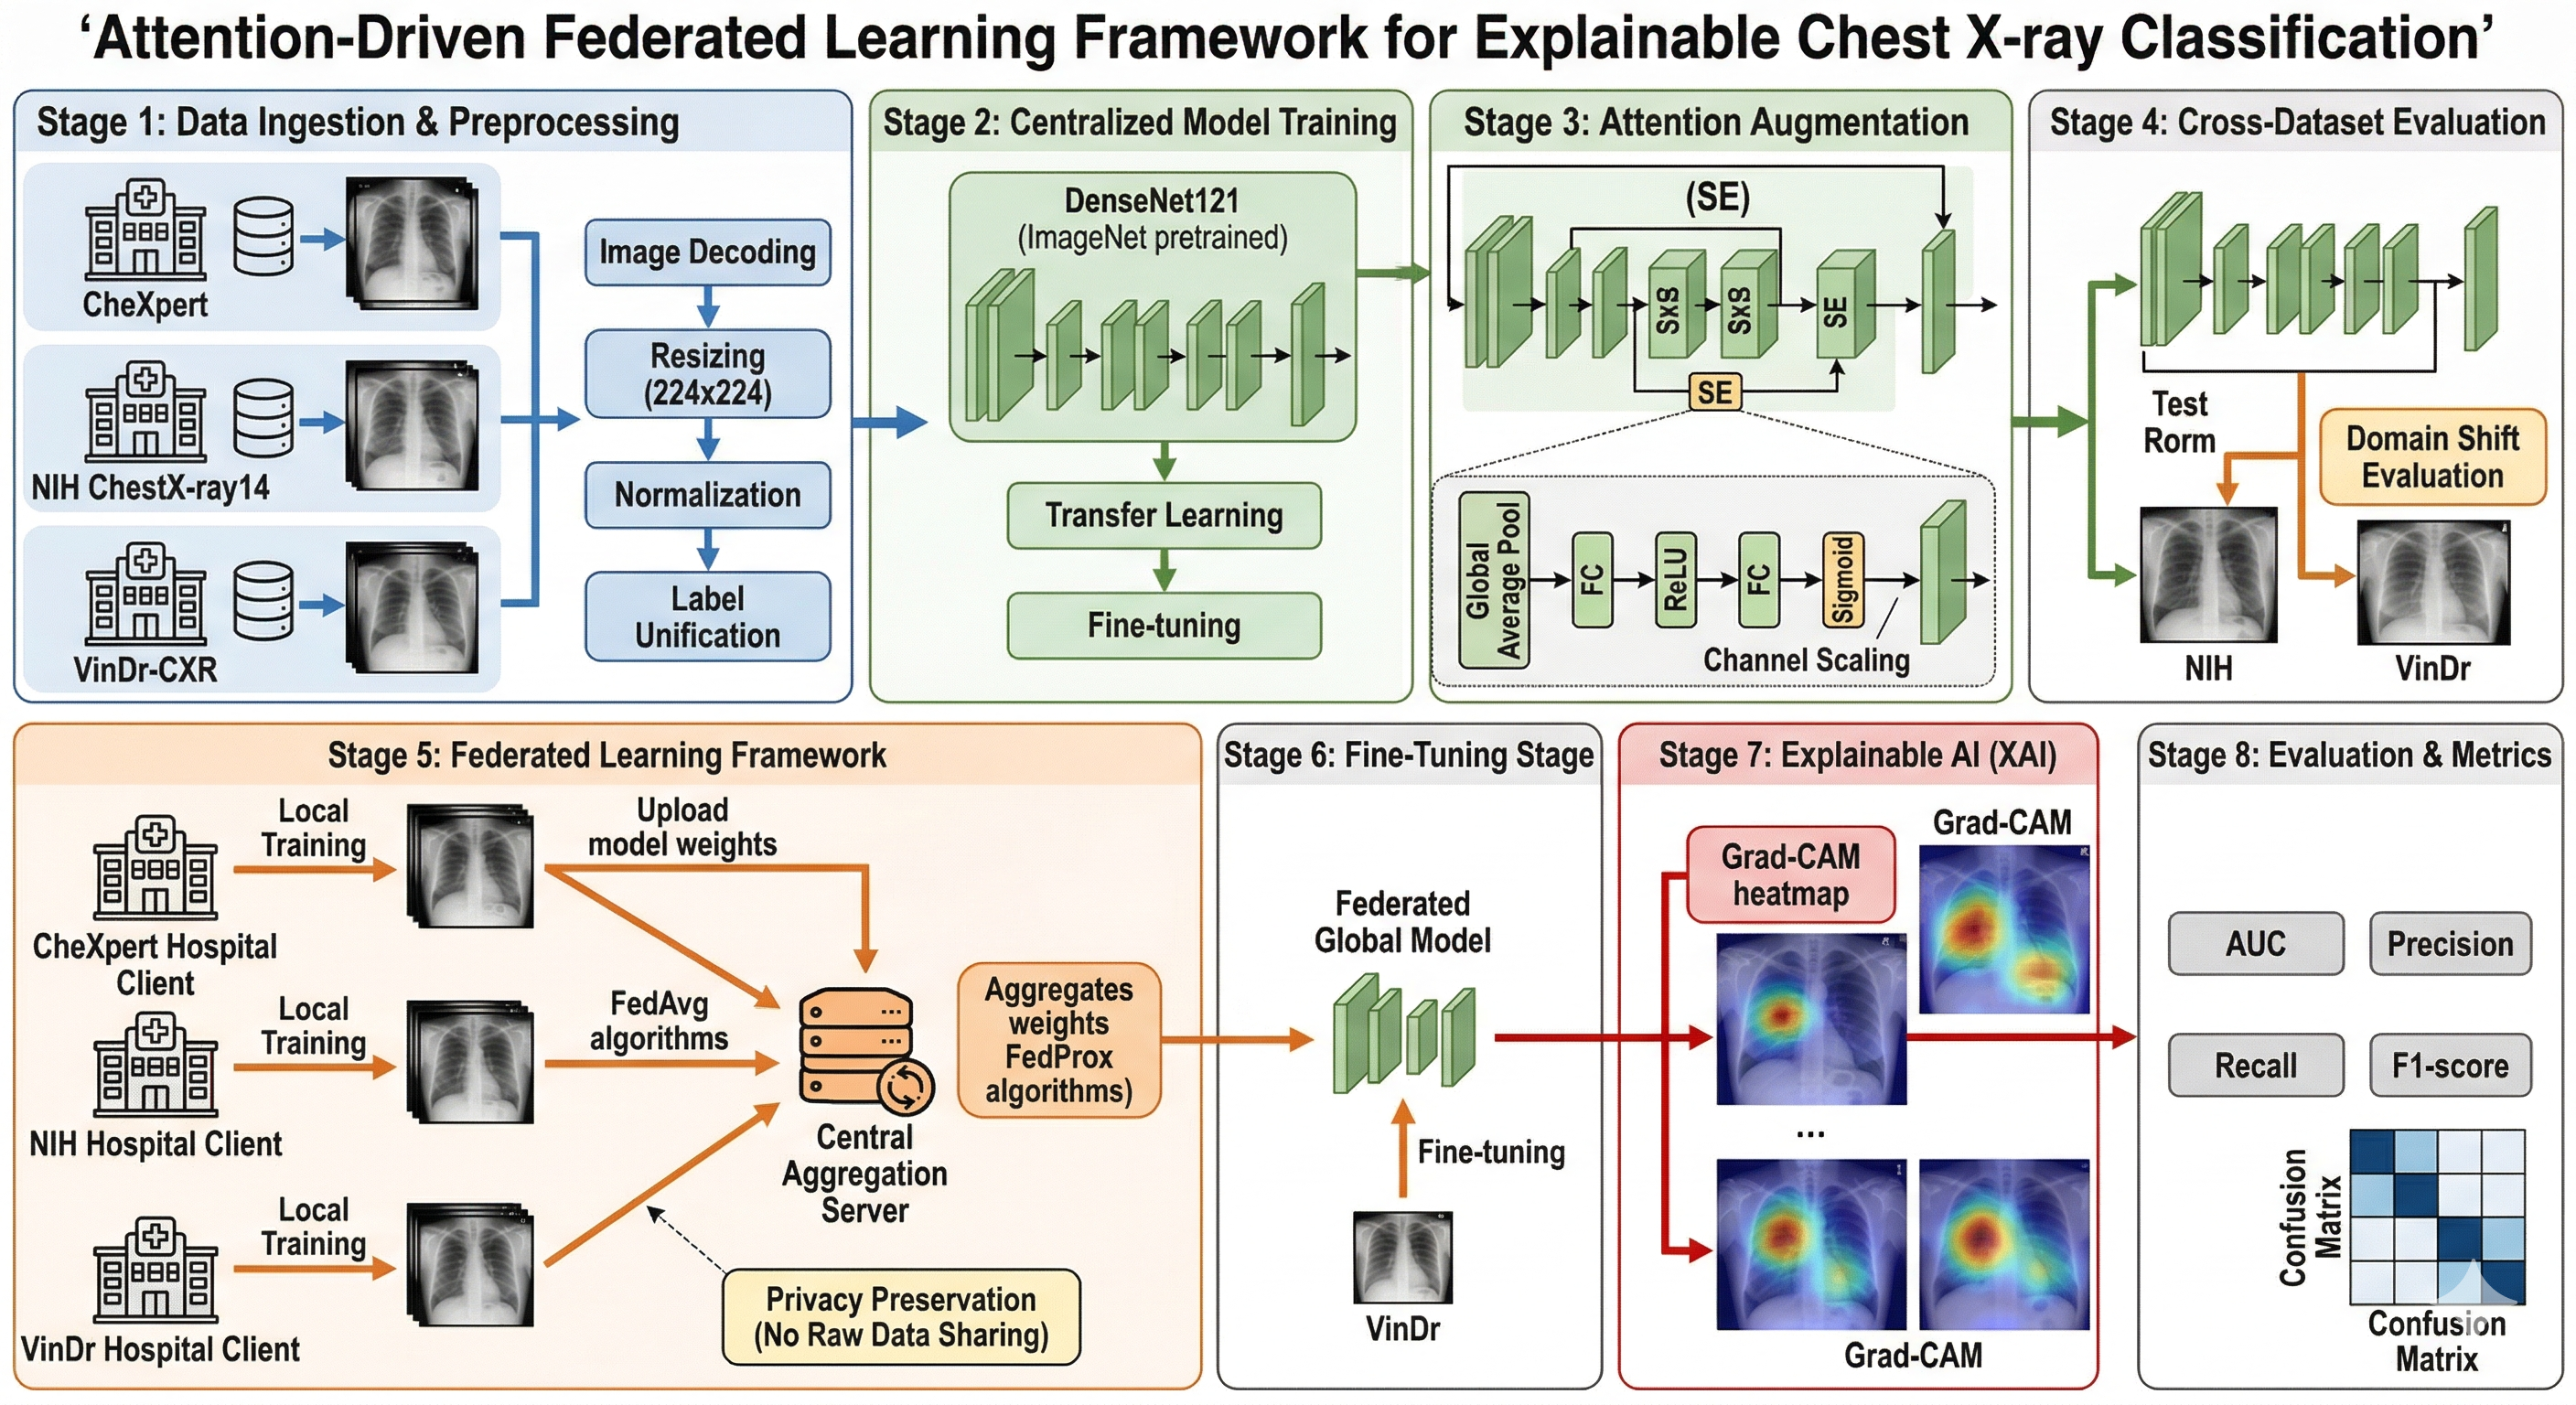
\includegraphics[width=\textwidth]{../fig/Project.png}
}{
\fbox{\parbox{0.9\textwidth}{\centering
\textbf{Architecture figure placeholder}\\
Insert the final project-specific architecture diagram here.
}}
}
\caption{Detailed architectural schematic illustrating the end-to-end data flow, from raw chest X-ray ingestion, through local SE-DenseNet121 optimization across heterogeneous client nodes, to global parameter aggregation and subsequent Grad-CAM explainability.}
\label{fig:system_architecture}
\end{figure}

\section{Data Pipeline and Distribution Strategy}

The foundation of any robust deep learning system is its data pipeline. The primary dataset utilized for model derivation is the RSNA Pneumonia Detection Challenge dataset, a globally recognized benchmark comprising tens of thousands of expertly annotated frontal chest radiographs.

\subsection{Preprocessing and Augmentation}
Raw medical images are inherently noisy and highly variable in resolution. The data pipeline standardizes this by employing bilinear interpolation to resize all images to a uniform tensor shape of $3 \times 224 \times 224$. To accelerate convergence and ensure the network weights are updated uniformly, z-score normalization is applied across all channels using the established ImageNet statistical means ($[0.485, 0.456, 0.406]$) and standard deviations ($[0.229, 0.224, 0.225]$).

During the local client training phases, the pipeline injects stochastic augmentations to artificially diversify the data. This includes random horizontal flips (mirroring the anatomical symmetry of the lungs), constrained rotations ($\pm 10$ degrees, to account for slight patient misalignment during scanning), and subtle brightness/contrast modulations. Crucially, these augmentations are strictly disabled during validation and testing to ensure deterministic and comparable evaluation metrics.

\subsection{Simulating Federated Heterogeneity}
To mimic a realistic multi-institutional deployment, the RSNA training corpus is partitioned into three discrete client datasets ($C_1, C_2, C_3$). Rather than an unrealistic uniform distribution, a Dirichlet distribution parameterized by $\alpha = 0.5$ is utilized. This explicitly introduces statistical heterogeneity (non-IID characteristics) into the client datasets, meaning one simulated hospital might see a disproportionately high rate of positive pneumonia cases compared to another, thereby providing a rigorous stress test for the federated optimization algorithms.

The entirely independent Labeled Chest X-ray Images dataset is held in strict quarantine from the training logic, serving exclusively as the final, unbiased arbiter of cross-domain generalizability.

\section{Neural Architecture: SE-DenseNet121}

The classification engine is a heavily modified DenseNet121 architecture. The standard DenseNet achieves exceptional parameter efficiency through its dense blocks, where the feature maps of all preceding layers are concatenated as inputs into all subsequent layers. This enforces a continuous flow of gradients and robust feature propagation.

To elevate the network's diagnostic capability, Squeeze-and-Excitation (SE) attention modules are strategically grafted into the architecture immediately following each of the four dense blocks, prior to the transition layers. As formulated in Chapter 3, these SE blocks act as a self-attention mechanism. They computationally "squeeze" the spatial dimensions into a channel descriptor and use a fully connected bottleneck to "excite" or scale the feature maps based on their learned relevance. In the context of pneumonia detection, this allows the network to suppress heavily activated channels corresponding to normal bone structure (like ribs) and amplify channels responding to opaque pulmonary infiltrates.

The final classification head consists of a 2D Global Average Pooling layer to collapse the spatial dimensions, feeding into a fully connected dense layer initialized with Xavier uniform weights, culminating in a Sigmoid activation function to output a continuous probability score bounded between $[0, 1]$.

\section{Implementation of Federated Optimization Algorithms}

The federated training loop is the orchestrating protocol of the system. The procedure operates over $T = 50$ maximum communication rounds.

\subsection{The FedAvg Protocol}
In the FedAvg implementation, the central server broadcasts the current global model weights $w^t$. Each client initializes its local PyTorch model with these weights and executes the local training loop for $E = 2$ epochs using the Adam optimizer. The objective function is the class-weighted Binary Cross-Entropy (BCE) loss, ensuring the optimizer does not become biased toward the numerically dominant 'normal' class. After the epochs complete, the clients serialize their state dictionaries and transmit them to the server logic, which executes a precise, sample-size-weighted matrix addition to derive $w^{t+1}$.

\subsection{The FedProx Protocol}
The FedProx implementation shares the identical network architecture, communication round structure, and aggregation logic as FedAvg, ensuring a perfectly controlled experimental setup. The critical divergence lies within the local training loop's objective function. 

During the PyTorch backpropagation step, the algorithm retrieves the globally broadcasted weights $w^t$ (which are detached from the current computational graph). It then calculates the L2 norm (Euclidean distance) between the currently optimizing local weights $w$ and the global weights $w^t$. This scalar distance is multiplied by $\frac{\mu}{2}$ (where $\mu = 0.01$) and added to the standard class-weighted BCE loss. The optimizer therefore computes gradients that not only minimize classification error but actively resist deviating too far from the global consensus, thereby mathematically anchoring the learning process against client drift.

\begin{table}[H]
\centering
\caption{Hyperparameter Configuration for Federated Optimization}
\label{tab:training_config}
\begin{tabular}{p{5.5cm}p{6.5cm}}
\toprule
\textbf{Hyperparameter} & \textbf{Configured Value} \\
\midrule
Base Neural Architecture & DenseNet121 (Pretrained on ImageNet) \\
Attention Mechanism & Squeeze-and-Excitation (SE) Blocks \\
Optimization Algorithm & Adam (Adaptive Moment Estimation) \\
Base Learning Rate & $1 \times 10^{-4}$ \\
Weight Decay (L2 Penalty) & $1 \times 10^{-4}$ \\
Learning Rate Scheduler & ReduceLROnPlateau (Factor: 0.1, Patience: 3) \\
Batch Size & 32 (Constrained by 16GB VRAM) \\
Number of Simulated Clients ($K$) & 3 \\
Local Training Epochs ($E$) & 2 per communication round \\
Maximum Global Rounds ($T$) & 50 (Subject to Early Stopping) \\
FedProx Regularization ($\mu$) & 0.01 \\
Aggregation Methods Executed & FedAvg, FedProx \\
\bottomrule
\end{tabular}
\end{table}

\section{Explainability Engine (Grad-CAM)}

The Explainability Engine operates post-training as a critical diagnostic tool. It is implemented by registering forward and backward hooks into the final convolutional layer of the SE-DenseNet121 architecture. 

During the forward pass of a test image, the engine caches the high-dimensional feature activations. During the backward pass, initiated by forcing a gradient of $1$ on the target 'pneumonia' class node, the engine intercepts and caches the gradients flowing back into that specific convolutional layer. 

As detailed in the mathematical formulation, these gradients are spatially pooled to derive importance weights for each channel. The cached feature activations are then multiplied by these weights. The resulting tensor is collapsed across the channel dimension and passed through a ReLU activation to discard negative influences. This raw heatmap is then normalized between $[0, 1]$, color-mapped using a jet or inferno colormap via OpenCV, upsampled using bilinear interpolation to $224 \times 224$, and blended with the original grayscale radiograph to produce the final, clinically interpretable visual explanation.
% ==========================================================================
% CHAPTER 6: RESULTS AND DISCUSSION
% ==========================================================================
\chapter{Results and Discussion}

\section{Experimental Configuration and Baselines}

To ensure a rigorous and scientifically valid comparison, the experimental framework was designed to eliminate confounding variables. Both the FedAvg and FedProx models were trained utilizing the exact identical SE-DenseNet121 architecture, initialized with the same random seed (42), and subjected to the same simulated Dirichlet non-IID data distribution across the three simulated clients. 

Furthermore, to contextualize the performance of the federated models, two centralized baseline models were trained on the aggregated RSNA training dataset: a standard DenseNet121, and the SE-enhanced DenseNet121. These centralized models serve as the theoretical "upper bound" of performance, representing the accuracy achievable if privacy constraints were entirely ignored and all patient data was pooled into a single repository.

\section{Analysis of Internal Performance on the RSNA Dataset}

The internal testing phase evaluates the models on a held-out test partition of the RSNA dataset, representing data drawn from the exact same clinical distribution as the training data. The comprehensive results are detailed in Table~\ref{tab:rsna_results}.

\begin{table}[H]
\centering
\caption{Comprehensive Performance Metrics on the Internal RSNA Test Set}
\label{tab:rsna_results}
\begin{tabular}{lccccc}
\toprule
\textbf{Model Architecture / Protocol} & \textbf{Accuracy} & \textbf{Precision} & \textbf{Recall} & \textbf{F1-Score} & \textbf{AUC-ROC}\\
 & (\%) & (\%) & (\%) & (\%) & (\%)\\
\midrule
Centralized Standard DenseNet121 & 83.14 & 61.18 & 68.85 & 64.79 & 88.54\\
Centralized SE-DenseNet121 (Upper Bound) & \textbf{83.99} & \textbf{63.41} & 68.40 & 65.81 & 88.50\\
Federated SE-DenseNet121 (FedAvg) & 82.49 & 58.96 & 73.28 & 65.35 & 88.52\\
Federated SE-DenseNet121 (FedProx) & 82.16 & 57.79 & \textbf{77.27} & \textbf{66.13} & \textbf{88.63}\\
\bottomrule
\end{tabular}
\end{table}

The data reveals several critical insights. First, the centralized SE-DenseNet121 achieves the highest overall accuracy (83.99\%) and precision (63.41\%), validating the efficacy of the attention mechanism. Crucially, however, the federated models perform remarkably well, trailing the centralized upper bound by a mere $1-1.5\%$ in overall accuracy. This minimal degradation strongly validates the federated learning hypothesis: we can achieve near-centralized diagnostic performance without ever compromising the localized privacy of the raw X-ray data.

When comparing the two federated strategies, FedAvg achieves a slightly higher accuracy (82.49\%) compared to FedProx (82.16\%). However, accuracy alone is a deceptive metric in clinical diagnostics, especially given the class imbalance typical in medical datasets. In the context of pneumonia detection, Recall (Sensitivity) is arguably the paramount metric; failing to detect a true positive (a false negative) can have severe, life-threatening consequences for the patient, whereas a false positive merely triggers a secondary review by a radiologist. 

Here, the advantage of FedProx becomes evident. FedProx achieves a significantly higher recall (77.27\%) compared to FedAvg (73.28\%). This means the FedProx model is substantially better at identifying actual pneumonia cases. While this heightened sensitivity comes at the cost of a slight drop in precision (more false positives), the resulting F1-Score (the harmonic mean of precision and recall) and the overall AUC-ROC (88.63\%) dictate that FedProx offers a more balanced and clinically desirable risk profile.

\section{Cross-Domain Generalization on the External Dataset}

The true litmus test for any clinical AI model is its capacity to generalize to entirely unseen data distributions. To assess this, the fully trained global models were deployed, without any fine-tuning or transfer learning, against the independent Labeled Chest X-ray Images dataset. The results, presented in Table~\ref{tab:external_results}, highlight a stark divergence in algorithmic robustness.

\begin{table}[H]
\centering
\caption{Zero-Shot External Evaluation (Cross-Domain Generalization)}
\label{tab:external_results}
\begin{tabular}{lccccc}
\toprule
\textbf{Model Architecture / Protocol} & \textbf{Accuracy} & \textbf{Precision} & \textbf{Recall} & \textbf{F1-Score} & \textbf{AUC-ROC}\\
 & (\%) & (\%) & (\%) & (\%) & (\%)\\
\midrule
Centralized Standard DenseNet121 & 53.20 & 99.00 & 25.38 & 40.41 & 79.80\\
Centralized SE-DenseNet121 & 45.99 & 98.18 & 13.85 & 24.27 & 88.82\\
Federated SE-DenseNet121 (FedAvg) & 53.69 & \textbf{99.03} & 26.15 & 41.38 & 88.88\\
Federated SE-DenseNet121 (FedProx) & \textbf{70.51} & 96.82 & \textbf{54.62} & \textbf{69.84} & \textbf{90.35}\\
\bottomrule
\end{tabular}
\end{table}

Under the stress of domain shift---caused by different X-ray scanners, diverse patient demographics, and varying radiological protocols---the FedAvg model collapses. While its precision remains anomalously high (indicating it is very conservative), its recall plummets to a catastrophic 26.15\%. In a clinical setting, deploying this FedAvg model would mean missing nearly three-quarters of all actual pneumonia cases, rendering it highly dangerous and effectively useless. 

In sharp contrast, the FedProx model demonstrates profound resilience. It maintains an accuracy of 70.51\% and more than doubles the recall of FedAvg, reaching 54.62\%. Consequently, its F1-Score surges to 69.84\%, and its AUC-ROC breaks the 90\% threshold (90.35\%). This data conclusively proves the core hypothesis: the proximal regularization term in FedProx not only mitigates client drift during training but forces the network to learn generalized, invariant anatomical features rather than overfitting to the idiosyncratic statistical noise of the local training environments.

\section{Convergence and Stability Analysis}

Analyzing the global validation loss curves provides insight into the optimization dynamics of the two algorithms. Both methods exhibit stable convergence, but their trajectories differ. FedAvg exhibits greater volatility in its validation loss during the initial 15 communication rounds, indicative of the divergent local models violently clashing during the aggregation phase. It requires approximately 30-35 rounds to reach its optimal early-stopping point.

FedProx, constrained by the proximal penalty $\mu$, exhibits a noticeably smoother and more monotonic convergence trajectory. The regularization dampens the severe oscillations during aggregation, allowing FedProx to reach stable, near-optimal performance by round 20. This accelerated convergence profile translates directly to reduced computational overhead and, more importantly, minimized communication bandwidth requirements between the hospitals and the central server, a critical logistical factor in real-world federated deployments.

\begin{figure}[H]
\centering
\IfFileExists{FedAvg/graph_global_val_accuracy_loss_densenet_se_fedavg.png}{
\includegraphics[width=0.85\linewidth]{FedAvg/graph_global_val_accuracy_loss_densenet_se_fedavg.png}
}{
\fbox{\parbox{0.8\linewidth}{\centering Insert FedAvg global validation accuracy/loss figure}}
}
\caption{Global validation convergence trajectory for FedAvg, demonstrating higher initial volatility.}
\label{fig:fedavg_training}
\end{figure}

\begin{figure}[H]
\centering
\IfFileExists{FedProx/graph_global_val_accuracy_loss_densenet_se_fedprox.png}{
\includegraphics[width=0.85\linewidth]{FedProx/graph_global_val_accuracy_loss_densenet_se_fedprox.png}
}{
\fbox{\parbox{0.8\linewidth}{\centering Insert FedProx global validation accuracy/loss figure}}
}
\caption{Global validation convergence trajectory for FedProx, illustrating smoother and more rapid stabilization due to proximal regularization.}
\label{fig:fedprox_training}
\end{figure}


\section{Clinical Interpretability via Grad-CAM}

The quantitative metrics prove the model is accurate, but the Grad-CAM visualizations prove whether it is logically sound. By projecting the final convolutional gradients back onto the source radiograph, we can clinically audit the model's 'attention'.

\subsection{True Positives and True Negatives}
As demonstrated in Figures \ref{fig:gradcam_normal} and \ref{fig:gradcam_pneumonia}, for correctly classified Normal scans, the Grad-CAM heatmaps typically exhibit a diffuse, low-intensity activation pattern across the entire lung cavity, indicating the model correctly finds no localized region of interest to trigger a positive classification. Conversely, for True Positive pneumonia scans, the heatmaps showcase intense, highly localized 'hotspots' (red/orange regions). Crucially, these hotspots consistently align with anatomically valid pulmonary regions where radiopacities, consolidations, or infiltrates are visible to the human eye, thereby validating that the SE-DenseNet121 is relying on genuine pathological indicators rather than artifactual noise.

\subsection{Analyzing Misclassifications}
The true value of XAI often lies in analyzing model failures. Figure \ref{fig:gradcam_incorrect} illustrates representative misclassifications. In certain False Positive instances, the Grad-CAM heatmap reveals strong activations outside the pulmonary cavity, focusing erroneously on prominent clavicles, overlapping rib shadows, or external medical artifacts (like ECG leads or pacemakers). This transparency is vital; a radiologist reviewing a False Positive flagged by the AI can instantly dismiss the prediction by observing that the Grad-CAM heatmap is focusing on irrelevant anatomy, thereby mitigating the risk of automation bias and ensuring patient safety.

\begin{figure}[H]
\centering
\IfFileExists{FedAvg/correct_normal.png}{
\includegraphics[width=0.48\linewidth]{FedAvg/correct_normal.png}
\hfill
}{
\fbox{\parbox{0.43\linewidth}{\centering Insert FedAvg correct-normal Grad-CAM}}
\hfill
}
\IfFileExists{FedProx/gradcam_densenet_se_fedprox_correct_normal_1.png}{
\includegraphics[width=0.48\linewidth]{FedProx/gradcam_densenet_se_fedprox_correct_normal_1.png}
}{
\fbox{\parbox{0.43\linewidth}{\centering Insert FedProx correct-normal Grad-CAM}}
}
\caption{Grad-CAM analysis of True Negatives: The models display diffuse, low-confidence activations, correctly identifying the absence of localized pathology.}
\label{fig:gradcam_normal}
\end{figure}

\begin{figure}[H]
\centering
\IfFileExists{FedAvg/correct_pneumonia.png}{
\includegraphics[width=0.48\linewidth]{FedAvg/correct_pneumonia.png}
\hfill
}{
\fbox{\parbox{0.43\linewidth}{\centering Insert FedAvg correct-pneumonia Grad-CAM}}
\hfill
}
\IfFileExists{FedProx/gradcam_densenet_se_fedprox_correct_pneumonia_1.png}{
\includegraphics[width=0.48\linewidth]{FedProx/gradcam_densenet_se_fedprox_correct_pneumonia_1.png}
}{
\fbox{\parbox{0.43\linewidth}{\centering Insert FedProx correct-pneumonia Grad-CAM}}
}
\caption{Grad-CAM analysis of True Positives: Intense focal activations correctly align with visual evidence of pulmonary consolidations.}
\label{fig:gradcam_pneumonia}
\end{figure}

\begin{figure}[H]
\centering
\IfFileExists{FedAvg/incorrect_prediction.png}{
\includegraphics[width=0.48\linewidth]{FedAvg/incorrect_prediction.png}
\hfill
}{
\fbox{\parbox{0.43\linewidth}{\centering Insert FedAvg misclassified Grad-CAM}}
\hfill
}
\IfFileExists{FedProx/gradcam_densenet_se_fedprox_incorrect_prediction_1.png}{
\includegraphics[width=0.48\linewidth]{FedProx/gradcam_densenet_se_fedprox_incorrect_prediction_1.png}
}{
\fbox{\parbox{0.43\linewidth}{\centering Insert FedProx misclassified Grad-CAM}}
}
\caption{XAI Audit of Misclassifications: Heatmaps reveal erroneous model attention on non-pulmonary structures or image artifacts, providing critical context for clinical override.}
\label{fig:gradcam_incorrect}
\end{figure}


% ==========================================================================
% CHAPTER 7: CONCLUSION
% ==========================================================================
\chapter{Conclusion}

This research set out to rigorously design, implement, and evaluate a comprehensive, privacy-preserving computational framework capable of automated pneumonia detection from complex chest radiographs. The resulting architecture successfully synthesizes the potent feature-extraction capabilities of an ImageNet-pretrained DenseNet121, the dynamic channel recalibration of Squeeze-and-Excitation (SE) attention modules, the decentralized data-privacy protocols of Federated Learning, and the clinical transparency afforded by Grad-CAM visual explanations.

The empirical data gathered from extensive simulations across three heterogeneous hospital clients yields several definitive conclusions. First, the project confirms that federated learning is a highly viable paradigm for medical imaging. The federated SE-DenseNet121 models achieved internal test accuracies exceeding 82\%, trailing the centralized, non-private baseline models by a statistically marginal degree. This demonstrates that we can unlock the collective intelligence of disparate medical datasets without ever compromising patient confidentiality or violating data localization policies.

The core investigative focus—the comparative analysis of the FedAvg and FedProx optimization algorithms—revealed critical insights for practical deployment. Within the controlled environment of the internal RSNA test set, both algorithms performed competitively, with FedProx demonstrating a slight, clinically beneficial bias toward higher recall (77.27\% vs 73.28\%). However, the zero-shot external evaluation on the independent Labeled Chest X-ray dataset categorically proved the superiority of the FedProx algorithm under conditions of domain shift. While FedAvg suffered a catastrophic collapse in recall (falling to 26.15\%), FedProx exhibited profound robustness, more than doubling the recall to 54.62\% and pushing the AUC-ROC beyond 90\%. This decisively concludes that the proximal regularization inherent to FedProx effectively anchors the local models, preventing overfitting to local statistical noise and yielding a generalized model far more resilient to the heterogeneity encountered in real-world clinical environments.

Furthermore, the integration of Grad-CAM transitioned the system from an opaque statistical engine to an auditable diagnostic support tool. The generated heatmaps consistently validated that the model’s successful predictions were driven by genuine pathological features, while simultaneously providing clinicians with the necessary visual context to safely identify and overrule algorithmic misclassifications.

In summation, this research proves that the integration of attention-enhanced neural architectures with advanced, proximally-regularized federated optimization and post-hoc explainability creates a highly robust, scalable, and trustworthy solution for collaborative medical AI, paving the way for next-generation diagnostic tools that respect both clinical accuracy and patient privacy.


% ==========================================================================
% CHAPTER 8: FUTURE WORK
% ==========================================================================
\chapter{Future Work}

While this framework establishes a highly robust foundation for privacy-preserving, interpretable pneumonia detection, the research landscape offers several critical vectors for future expansion and refinement:

\begin{enumerate}
    \item \textbf{Transition to Real-World Multi-Institutional Topologies:} The current framework relies on simulated client nodes partitioned from a central dataset. The immediate next phase must involve deploying the architecture across a genuine wide-area network, linking physically distinct, independent healthcare institutions. This will necessitate resolving real-world logistical challenges, including asynchronous communication protocols to handle network latency, robust fault tolerance mechanisms for client dropouts, and the standardization of disparate hospital IT infrastructures.

    \item \textbf{Integration of Cryptographic Privacy Guarantees:} Federated learning protects raw data but remains theoretically vulnerable to sophisticated model inversion attacks against the transmitted weight parameters. Future iterations must implement rigorous cryptographic layers. The integration of Formal Differential Privacy (DP), which injects mathematically calibrated noise into the client gradients, would provide provable privacy guarantees. Additionally, implementing Secure Multiparty Computation (SMPC) or Secure Aggregation protocols would ensure that the central server can only compute the synthesized global model without ever gaining the ability to inspect the individual updates from specific hospitals.

    \item \textbf{Expansion to Multi-Label and 3D Modalities:} The scope of this project was constrained to binary pneumonia classification from 2D frontal radiographs. Future research should extend the SE-DenseNet121 architecture, potentially modifying the classification head, to support multi-label thoracic disease detection (e.g., simultaneously identifying cardiomegaly, effusions, pneumothorax, and nodules). Furthermore, adapting the federated framework to process high-dimensional 3D imaging modalities, such as Computed Tomography (CT) scans, would drastically increase its diagnostic utility, albeit requiring significant research into communication-efficient gradient compression techniques.

    \item \textbf{Advanced Algorithmic Optimization:} While FedProx proved superior to FedAvg under heterogeneity, the field of federated optimization is rapidly evolving. Future studies should benchmark this framework against emerging, state-of-the-art algorithms such as SCAFFOLD (Stochastic Controlled Averaging), which utilizes control variates to actively correct for client drift, or FedNova, which normalizes the local updates based on the varying number of local steps taken by heterogeneous clients, potentially unlocking even higher levels of cross-domain generalizability.
\end{enumerate}


% ==========================================================================
% REFERENCES
% ==========================================================================
\newpage
\addcontentsline{toc}{chapter}{\numberline{}References}
\begin{thebibliography}{99}
\setstretch{1.5}

\bibitem{rajpurkar2017chexnet}
P. Rajpurkar \textit{et al.}, ``CheXNet: Radiologist-level pneumonia detection on chest X-rays with deep learning,'' \textit{arXiv preprint arXiv:1711.05225}, 2017.

\bibitem{huang2017densely}
G. Huang, Z. Liu, L. Van Der Maaten, and K. Q. Weinberger, ``Densely connected convolutional networks,'' in \textit{Proc. IEEE Conf. Comput. Vis. Pattern Recognit. (CVPR)}, Honolulu, HI, USA, 2017, pp. 4700--4708.

\bibitem{mcmahan2017communication}
B. McMahan, E. Moore, D. Ramage, S. Hampson, and B. Ag{\"u}era y Arcas, ``Communication-efficient learning of deep networks from decentralized data,'' in \textit{Proc. 20th Int. Conf. Artificial Intelligence and Statistics (AISTATS)}, Fort Lauderdale, FL, USA, 2017, pp. 1273--1282.

\bibitem{li2020federated}
T. Li, A. K. Sahu, A. Talwalkar, and V. Smith, ``Federated optimization in heterogeneous networks,'' in \textit{Proc. Machine Learning and Systems (MLSys)}, vol. 2, 2020, pp. 429--450.

\bibitem{hu2018squeeze}
J. Hu, L. Shen, and G. Sun, ``Squeeze-and-excitation networks,'' in \textit{Proc. IEEE Conf. Comput. Vis. Pattern Recognit. (CVPR)}, Salt Lake City, UT, USA, 2018, pp. 7132--7141.

\bibitem{selvaraju2017gradcam}
R. R. Selvaraju, M. Cogswell, A. Das, R. Vedantam, D. Parikh, and D. Batra, ``Grad-CAM: Visual explanations from deep networks via gradient-based localization,'' in \textit{Proc. IEEE Int. Conf. Comput. Vis. (ICCV)}, Venice, Italy, 2017, pp. 618--626.

\bibitem{rieke2020}
N. Rieke \textit{et al.}, ``The future of digital health with federated learning,'' \textit{NPJ Digital Medicine}, vol. 3, no. 1, pp. 1--7, 2020.

\bibitem{sheller2020federated}
M. J. Sheller, G. A. Reina, B. Edwards, J. Martin, and S. Bakas, ``Federated learning in medicine: Facilitating multi-institutional collaborations without sharing patient data,'' \textit{Scientific Reports}, vol. 10, no. 1, p. 12598, 2020.

\bibitem{kaissis2020secure}
G. A. Kaissis, M. R. Makowski, D. R{\"u}ckert, and R. F. Braren, ``Secure, privacy-preserving and federated machine learning in medical imaging,'' \textit{Nature Machine Intelligence}, vol. 2, no. 6, pp. 305--311, 2020.

\bibitem{shih2019rsna}
G. Shih \textit{et al.}, ``Augmenting the National Institutes of Health chest radiograph dataset with expert annotations of possible pneumonia,'' \textit{Radiology: Artificial Intelligence}, vol. 1, no. 1, p. e180041, 2019.

\end{thebibliography}

\end{document}
